\chapter{TrueCrypt}
\paragraph{}
TrueCrypt je šifrovací program umožňujúci používateľovi na základe ním zvoleného hesla vytvoriť šifrovaný disk. Taktiež používateľovi umožňuje vytvorenie virtuálneho šifrovaného disku, ktorý bude následne uložený v súbore na fyzickom disku. Vývoj tohto programu bol ukončený v roku 2014 a podľa autorov nie je bezpečný, nakoľko jeho implementácia môže obsahovať bezpečnostné chyby. Následný bezpečnostný audit tohto programu neukázal žiadne závažné bezpečnostné chyby v jeho základnom návrhu. 

\paragraph{}
V septembri 2015 prišiel James Forshaw s informáciou o 2 chybách vo ovládači Windows-u, ktorý používa program TrueCrypt. Jedna z chýb umožňuje útočníkovi plný prístup k zašifrovaným partíciam iných používateľov, ktoré sú na tom istom počítači \cite{issue1}. Druhá, závažnejšia chyba umožňuje útočníkovi prístup k zvýšeným právam zneužitím tvorby symbolického odkazu na písmená diskov \cite{issue2}. Obe tieto chyby sa dokážu prejaviť až počas behu samotného programu. Preto ich v tejto práci používať nebudeme, nakoľko pre náš algoritmus nie je potrebné aby TrueCrypt bežal.

\paragraph{}
Ako sme spomínali v úvode, program TrueCrypt slúži na zašifrovanie dát na používateľskom disku pomocou zvoleného hesla. K tomuto TrueCrypt používa niektorý zo~šifrovacích algoritmov medzi ktoré patrí AES, Serpent alebo Twofish. Keďže sa jedná o blokové šifry, TrueCrypt používa blokové šifry v XTS móde na šifrovanie objemu dát väčšieho ako je 1 blok šifry. TrueCrypt taktiež poskytuje možnosť vybrať si jednu z~podporovaných hešovacích funkcií ako RIPEMD-160, SHA-512 a Whirlpool.

\paragraph{}
Samotné šifrovanie partície prebieha vo viacerých fázach: 
\begin{itemize}
	\item Vygeneruje sa náhodný kľúč vhodný na šifrovanie pomocou zvoleného algoritmu. 
	\begin{itemize}
		\item V prípade XTS módu veľkosť kľúča zdvojnásobíme. Dôvodom je použitie 2 kľúčov pri šifrovaní v XTS móde ako je znázornené na obrázku \ref{fig:XTS}
	\end{itemize}
	\item Pomocou tohto kľúča sa zašifruje celá požadovaná partícia
	\item Vytvorí sa hlavička pre túto partíciu obsahujúca:
	\begin{itemize}
		\item Verziu programu TrueCrypt
		\item Verziu hlavičky
		\item ASCII reťazec `TRUE'
		\item Vygenerovaný kľúč použitý na zašifrovanie dát
		\item CRC-32 kontrolná suma kľúča
		\item CRC-32 kontrolná suma zvyšku hlavičky
	\end{itemize}
	\item Táto hlavička sa zašifruje pomocou kľúča vygenerovaného na základe používateľského hesla, ktoré nemusí byť vhodné na použitie ako šifrovací kľúč
	\begin{itemize}
		\item K heslu sa pripojí náhodný 512 bitový reťazec - kryptografická soľ
		\item Takto upravené heslo sa dá na vstup algoritmu PBKDF2
		\item Transformáciami pomocou hešovacích funkcií vznikne vhodný kľúč na šifrovanie
	\end{itemize}
	\item Vyššie vygenerovaná kryptografická soľ sa nezašifrovaná pridá pred hlavičku partície
\end{itemize}
Takto zašifrovaná partícia je nakoniec uložená na fyzickom disku v súboru obsahujúcom:
\begin{itemize}
	\item Kryptografickú soľ v nešifrovanej forme
	\item Šifrovanú hlavičku partície obsahujúcej kľúč použitý na šifrovanie dát
	\item Používateľom zvolené dáta zašifrované programom TrueCrypt
\end{itemize}

\begin{figure}[h]
    \centering
    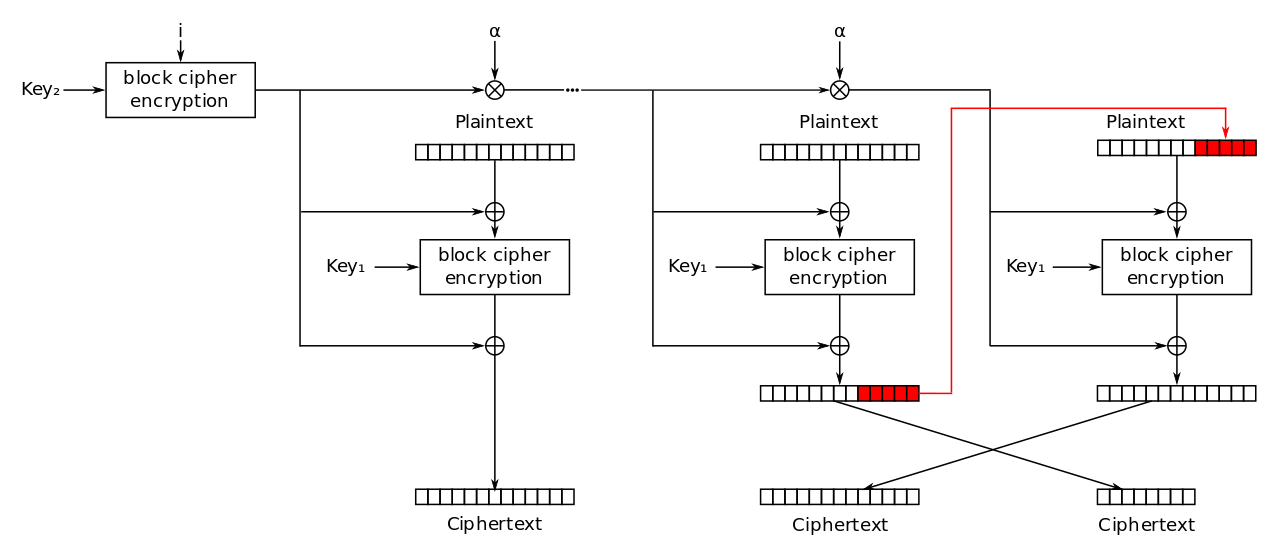
\includegraphics[width=1\textwidth]{XTS_mode_encryption}
    \caption{Schéma módu XTS}
    \label{fig:XTS}
\end{figure}

\paragraph{XTS mód}
Na obrázku \ref{fig:XTS} vidíme schému módu XTS pre blokové šifry. Základ tvorí mód XEX, ktorý bol navrhnutý na efektívne spracovanie za sebou nasledujúcich blokov vrámci dátového bloku napríklad diskového sektoru. Na schéme môžeme vidieť použitie dvoch rôznych kľúčov \(Key_1\) a \(Key_2\). Kvôli použitiu týchto kľúčov sa častokrát generuje šifrovací kľúč dvojnásobnej dĺžky, kedy sa následne prvá polovica použije ako \(Key_1\) a druhá ako \(Key_2\). Hodnota \(i\) vyjadruje číslo diskového sektoru, ktorý sa práve šifruje, zatiaľ čo \(\alpha\) je prvok z konečného poľa \(GF(2^128)\). Pre každý blok šifry sa spraví \(\alpha^j\), kde \(j\) je číslo bloku vrámci sektoru. Mód XTS prináša módu XEX podporu pre~sektory veľkosti nedeliteľnej veľkosťou bloku šifry. Ak posledný blok otvoreného textu nemá dostatočnú veľkosť, pridá sa k nemu potrebný počet bajtov predošlého zašifrovaného bloku. Po zašifrovaní takto upraveného otvoreného textu sa novo zašifrovaný blok vymení so zvyškom predposledného šifrovaného bloku, ako je znázornené na schéme.

\begin{listing}
\begin{minted}[linenos,
			   tabsize=2,
               numbersep=3pt,
               frame=single,
               framesep=2mm]{c++}
switch (pkcs5_prf)
{
	case RIPEMD160:
		derive_key_ripemd160 (keyInfo.userKey, keyInfo.keyLength,
						keyInfo.salt, PKCS5_SALT_SIZE,
						keyInfo.noIterations, dk, GetMaxPkcs5OutSize());
		break;

	case SHA512:
		derive_key_sha512 (keyInfo.userKey, keyInfo.keyLength, 
						keyInfo.salt, PKCS5_SALT_SIZE, 
						keyInfo.noIterations, dk, GetMaxPkcs5OutSize());
		break;

	case SHA1:
		// Deprecated/legacy
		derive_key_sha1 (keyInfo.userKey, keyInfo.keyLength,
						keyInfo.salt, PKCS5_SALT_SIZE, 
						keyInfo.noIterations, dk, GetMaxPkcs5OutSize());
		break;

	case WHIRLPOOL:
		derive_key_whirlpool (keyInfo.userKey, keyInfo.keyLength, 
						keyInfo.salt, PKCS5_SALT_SIZE, 
						keyInfo.noIterations, dk, GetMaxPkcs5OutSize());
		break;

	default:		
		// Unknown/wrong ID
		TC_THROW_FATAL_EXCEPTION;
}
\end{minted}
\caption{Ukážka kódu transformácie hesla na šifrovací kľúč}
\label{lst:tc1}
\end{listing}

\paragraph{}
Vďaka zdrojovým kódom voľne prístupným na internete, sme mali možnosť si ich prehliadnuť a hľadať v nich možnosť rýchleho overovania kandidátov na hľadané používateľské heslo. Našim cieľom pri tomto hľadaní bolo nájdenie časti kódu, ktorá je zodpovedná za prijatie používateľského vstupu a jeho následné spracovanie. Toto spracovanie zahŕňa transformáciu tohto vstupu na kľúč, ktorým sa program pokúsi rozšifrovať hlavičku partície \ref{lst:tc1}. Následne sa program posnaží rozšifrovať hlavičku pomocou tohto kľúču a overí, či dáta v nej dávajú zmysel. Toto zahŕňa overenie reťazca \emph{`TRUE'}, verzie hlavičky, minimálnej verzie programu a CRC-32 súm kľúčov a ostatných položiek \ref{lst:tc2}. Bohužiaľ vrámci tejto práce sme nemali čas izolovať minimálny kód potrebný na~úspešne fungovanie tohto overenia.

\begin{listing}
\begin{minted}[linenos,
			   tabsize=2,
               numbersep=3pt,
               frame=single,
               framesep=2mm]{c}
// Copy the header for decryption
memcpy (header, encryptedHeader, sizeof (header));

// Try to decrypt header 
DecryptBuffer (header + HEADER_ENCRYPTED_DATA_OFFSET,
			HEADER_ENCRYPTED_DATA_SIZE, cryptoInfo);

// Magic 'TRUE'
if (GetHeaderField32 (header, TC_HEADER_OFFSET_MAGIC) != 0x54525545)
	continue;

// Header version
headerVersion = GetHeaderField16 (header, TC_HEADER_OFFSET_VERSION);

if (headerVersion > VOLUME_HEADER_VERSION)
{
	status = ERR_NEW_VERSION_REQUIRED;
	goto err;
}

// Check CRC of the header fields
if (!ReadVolumeHeaderRecoveryMode
	&& headerVersion >= 4
	&& GetHeaderField32 (header, TC_HEADER_OFFSET_HEADER_CRC) != 
		GetCrc32 (header + TC_HEADER_OFFSET_MAGIC, 
		TC_HEADER_OFFSET_HEADER_CRC - TC_HEADER_OFFSET_MAGIC))
	continue;

// Required program version
cryptoInfo->RequiredProgramVersion = GetHeaderField16 (header, 
							TC_HEADER_OFFSET_REQUIRED_VERSION);
cryptoInfo->LegacyVolume = cryptoInfo->RequiredProgramVersion < 0x600;

// Check CRC of the key set
if (!ReadVolumeHeaderRecoveryMode
	&& GetHeaderField32 (header, TC_HEADER_OFFSET_KEY_AREA_CRC) != 
	GetCrc32 (header + HEADER_MASTER_KEYDATA_OFFSET,
			MASTER_KEYDATA_SIZE))
	continue;
\end{minted}
\caption{Ukážka kódu overenia správnosti hesla dešifrovaním hlavičky}
\label{lst:tc2}
\end{listing}

\paragraph{}
Zbytok tejto práce sa venuje generovaniu slovníka z ktorého budeme brať kandidátov na hľadané heslo.